% !TEX root = ../main.tex

\chapter{直流—交流：H 桥电流环}
\label{chap:hb}

\section{主电路}

实验三的对象是电压源型全桥驱动强感性负载、电流闭环的最小完整结构。四只 IGBT 分成两个桥臂，每只反并联一只二极管，C--E 之间并联 10 M$\Omega$ 缓冲电阻；桥臂中点 A、B 之间接 $R=0.2\ \Omega$、$L=20$~mH 的串联负载；直流侧为 2200~V 受控电压源。桥臂状态与输出电压的关系为
\begin{equation}
v\sub{AB}=(s_A-s_B)U\sub{dc},\qquad s_A,s_B\in\{0,1\},
\end{equation}
负载满足
\begin{equation}
L\frac{\dd i}{\dd t}=v\sub{AB}-Ri.
\label{eq:rl}
\end{equation}
式~\eqref{eq:rl} 不含任何控制假设，只要仿真中的 $v\sub{AB}$ 和 $i$ 满足它，功率级和测量链就是自洽的，后文把它作为校核工具。

模型顶层如图~\ref{fig:hb-model} 所示，按给定与使能、电流环与调制、功率级、监视记录四个功能区排列。功率级内部如图~\ref{fig:hb-power}(a) 所示。

\begin{figure}[htbp]
\centering
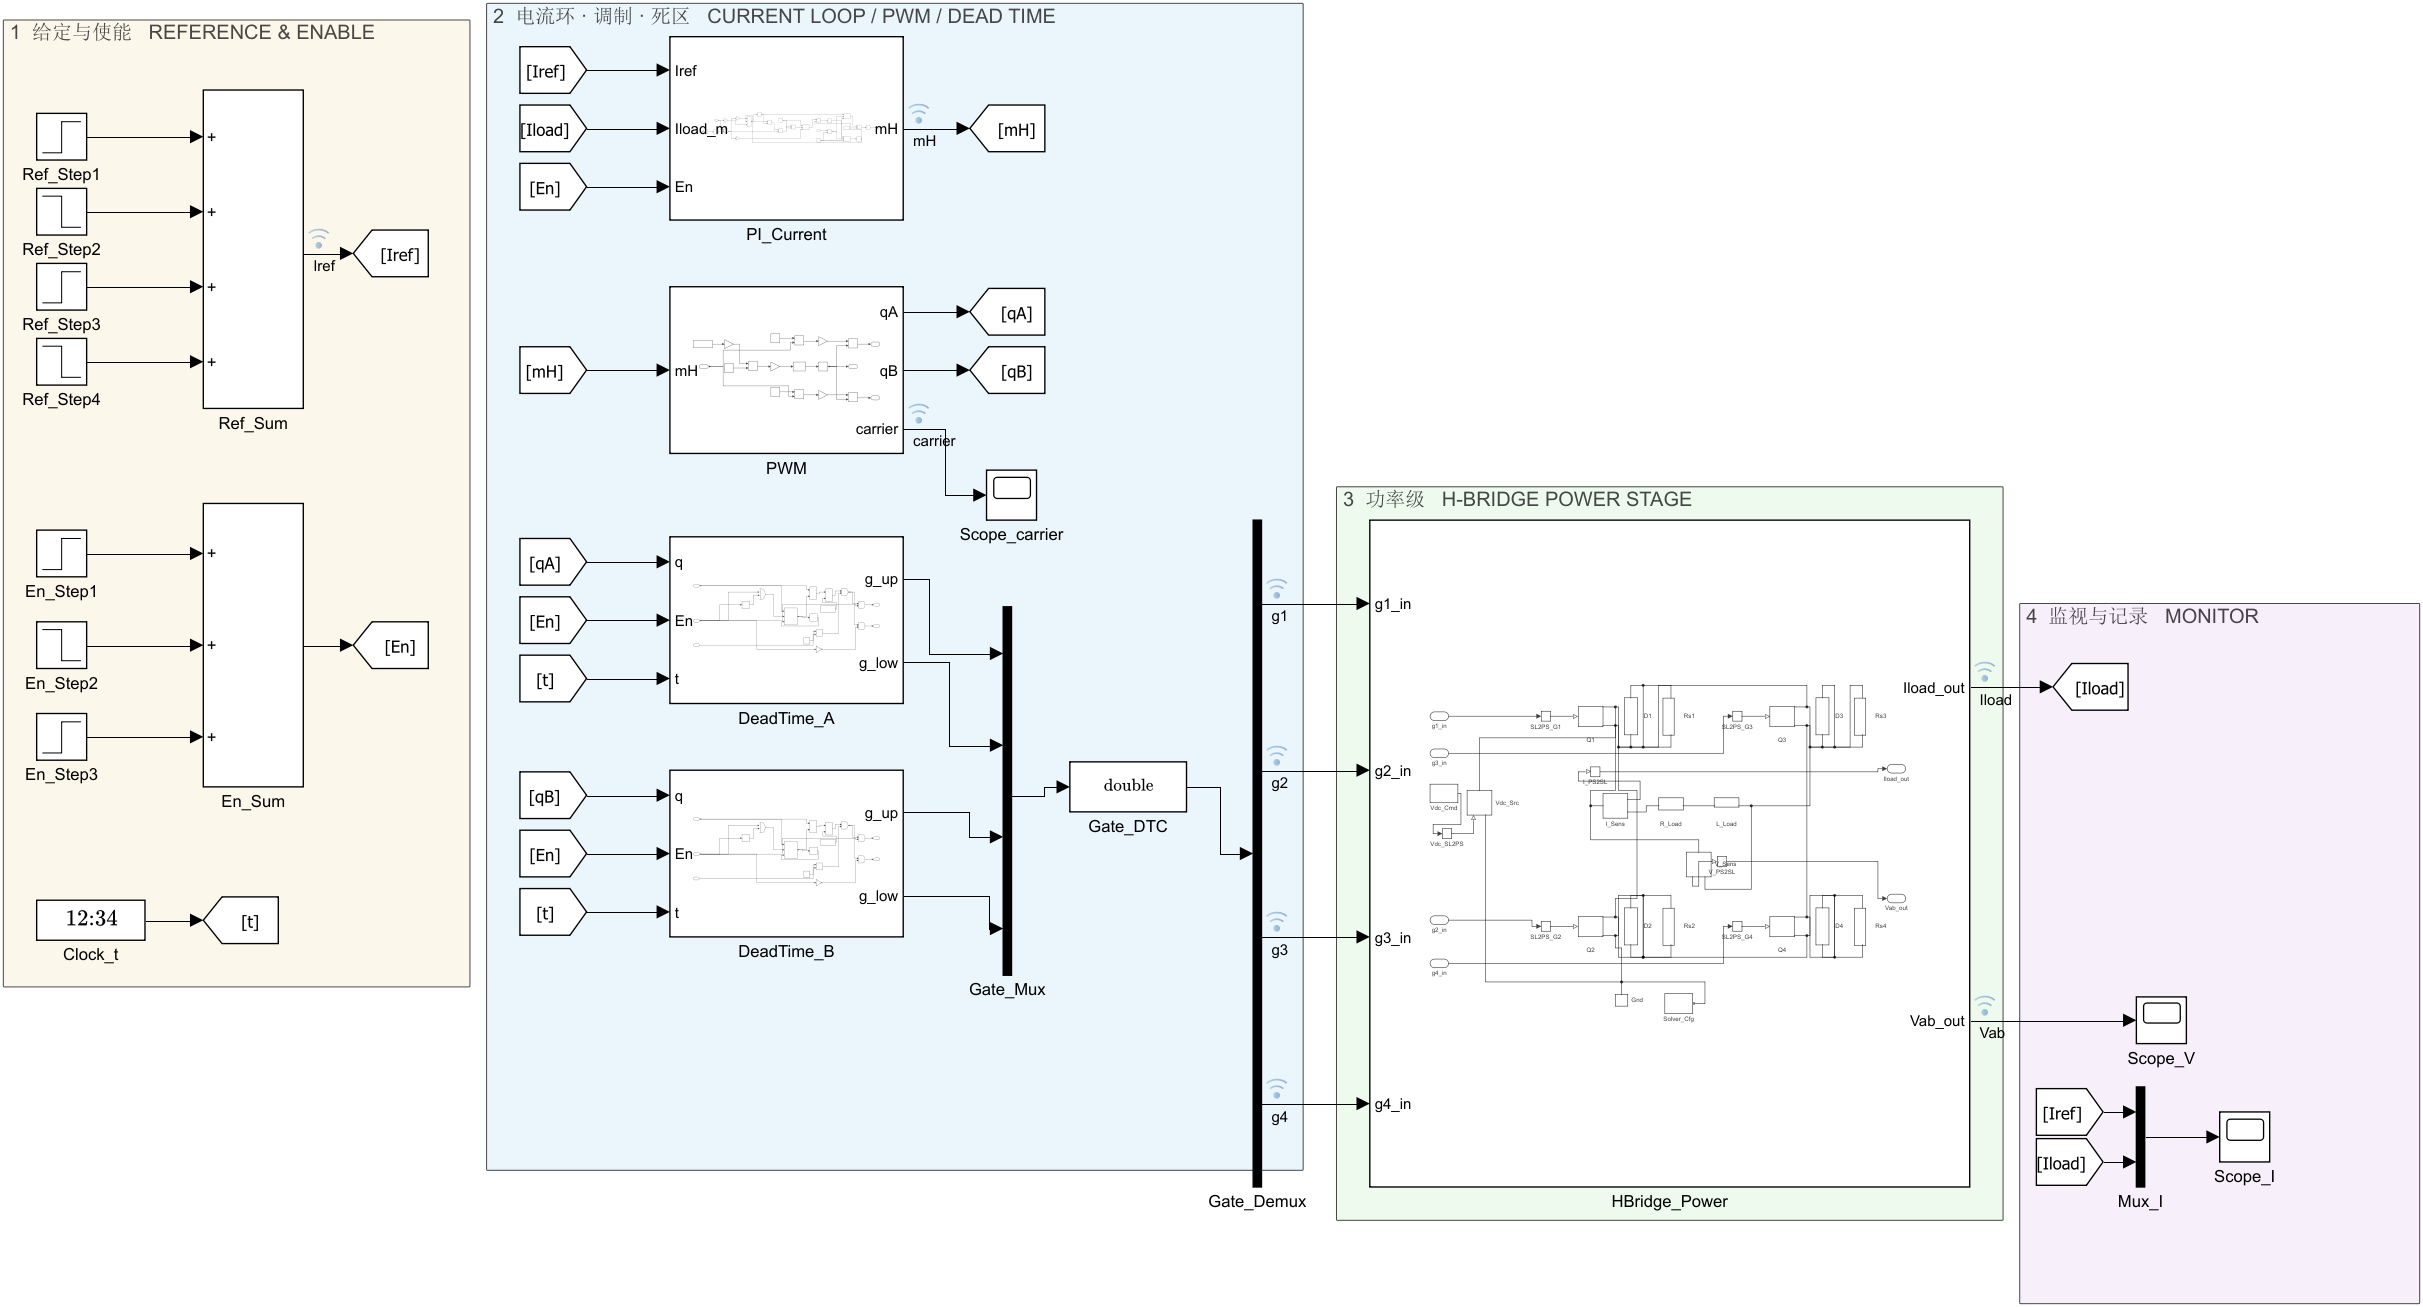
\includegraphics[width=0.74\linewidth]{hb_top.png}
\caption{H 桥模型顶层的四个功能分区（Simulink 原生视图）}
\label{fig:hb-model}
\end{figure}

\sidefig{native/model_hb_power.png}{native/model_deadtime.png}{H 桥模型子系统（Simulink 原生视图）：(a) \texttt{HBridge\_Power} 功率级，(b) 修正后的 \texttt{DeadTime\_A} 死区子系统}{fig:hb-power}

\section{电流环设计}

信号链为传感器、50~$\mu$s 零阶保持、50~$\mu$s 单位延迟和求差。误差分三路进入求和器：比例项 $K_pe$，积分增量 $K_iT_ce$（$T_c=50\ \mu$s），以及电阻压降前馈 $0.2i\sub{ref}$。求和结果限幅 $\pm400$~V，再除以 $U\sub{dc}$ 得到调制比 $m\sub{H}$，并限幅 $\pm0.95$。

参数按零极点对消整定，取 $K_p=\omega_cL$、$K_i=\omega_cR$，则开环传递函数为
\begin{equation}
G\sub{ol}(s)=\Bigl(K_p+\frac{K_i}{s}\Bigr)\frac{1}{Ls+R}=\frac{\omega_c}{s}.
\label{eq:loop}
\end{equation}
穿越频率取 100~Hz，得 $K_p=12.56637$~V/A、$K_i=125.66$~V/(A$\cdot$s)，$K_iT_c=6.2832\times10^{-3}$。抗饱和以限幅前后之差乘以电流误差为判据，结果大于零时把积分增量切为零。使能信号无效时积分状态清零、电压指令切零。图~\ref{fig:hb-pi}(a) 是 0.02~s 阶跃时的内部量：限幅前电压最高为 6268~V，被限到 400~V，积分状态在约 30~ms 的饱和区间内保持为零，退出饱和后才开始积累。

\section{单极性 PWM 与死区}

载波由数字时钟经取模和偏置得到 0--1 三角波，频率 2~kHz、周期 $T_s=500\ \mu$s。两桥臂占空比由同一个 $m\sub{H}$ 映射：
\begin{equation}
d_A=\frac{1+m\sub{H}}{2},\qquad d_B=\frac{1-m\sub{H}}{2},
\end{equation}
各自与同一载波比较。$m\sub{H}>0$ 时输出在 0 和 $+U\sub{dc}$ 之间切换，每个载波周期出现两个脉冲，平均输出电压为
\begin{equation}
\langle v\sub{AB}\rangle=U\sub{dc}\,m\sub{H}.
\label{eq:modlaw}
\end{equation}

死区按“请求变化后延迟 2~$\mu$s 再放行”实现：请求信号与其一拍延迟异或得到变化标志，记住最近一次变化的时刻，当前时间减去该时刻后与 2~$\mu$s 比较，结果再与使能相与（图~\ref{fig:hb-power}(b)）。图~\ref{fig:hb-pwm} 是 $+500$~A 平台 1~ms 的门极、负载电压和电流。负载 $L/R=0.1$~s 远大于载波周期，电流只呈锯齿状纹波，峰峰值 1.0--1.7~A。

原模型直接比较浮点时间差，实测换相间隔会出现 2--3~$\mu$s，只有最小值和中位数恒为 2~$\mu$s。修正版把经过时间先映射回 1~$\mu$s 时钟格点再与 2~$\mu$s 比较，重跑 0.42~s 全部工况后，两个桥臂各 1592 次完整换相的间隔全部为 2~$\mu$s（图~\ref{fig:hb-pi}(b)），门极序列中没有桥臂重叠导通。这一修正随后也用于第 \ref{chap:joint} 章的整机模型。

\begin{figure}[htbp]
\centering
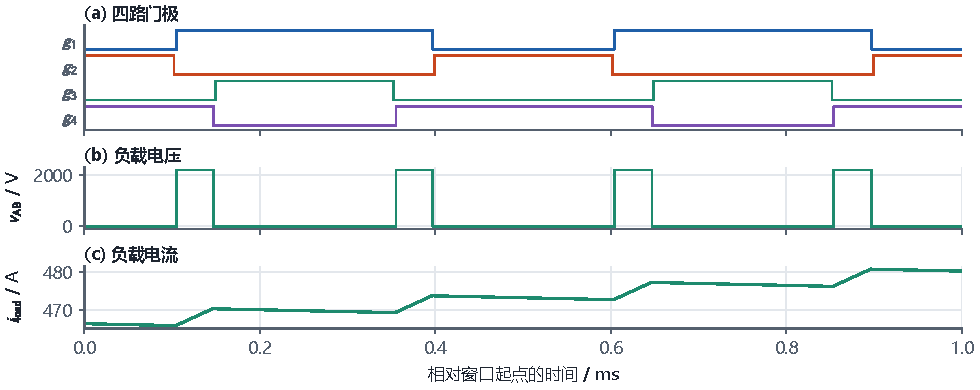
\includegraphics[width=\linewidth]{hb_pwm}
\caption{稳态 $+500$~A 平台：(a) 四路门极，(b) 负载电压，(c) 负载电流纹波}
\label{fig:hb-pwm}
\end{figure}

\twofig{native/hbridge_pi_saturation.pdf}{native/verified_deadtime.pdf}{MATLAB 原生波形：(a) 0.02~s 阶跃时限幅前后的电压指令与积分状态，(b) 修正版两桥臂门极的换相细节}{fig:hb-pi}

\section{五段给定的跟踪结果}

给定由四段阶跃叠加而成：0、$+500$、$-500$、$+300$~A，0.36~s 后回到 0；0.30--0.32~s 之间使能封锁，控制器复位。图~\ref{fig:hb-tracking} 是修正版模型的完整波形，表~\ref{tab:hb-track} 是原模型各段末 20\% 区间的统计。

\begin{figure}[htbp]
\centering
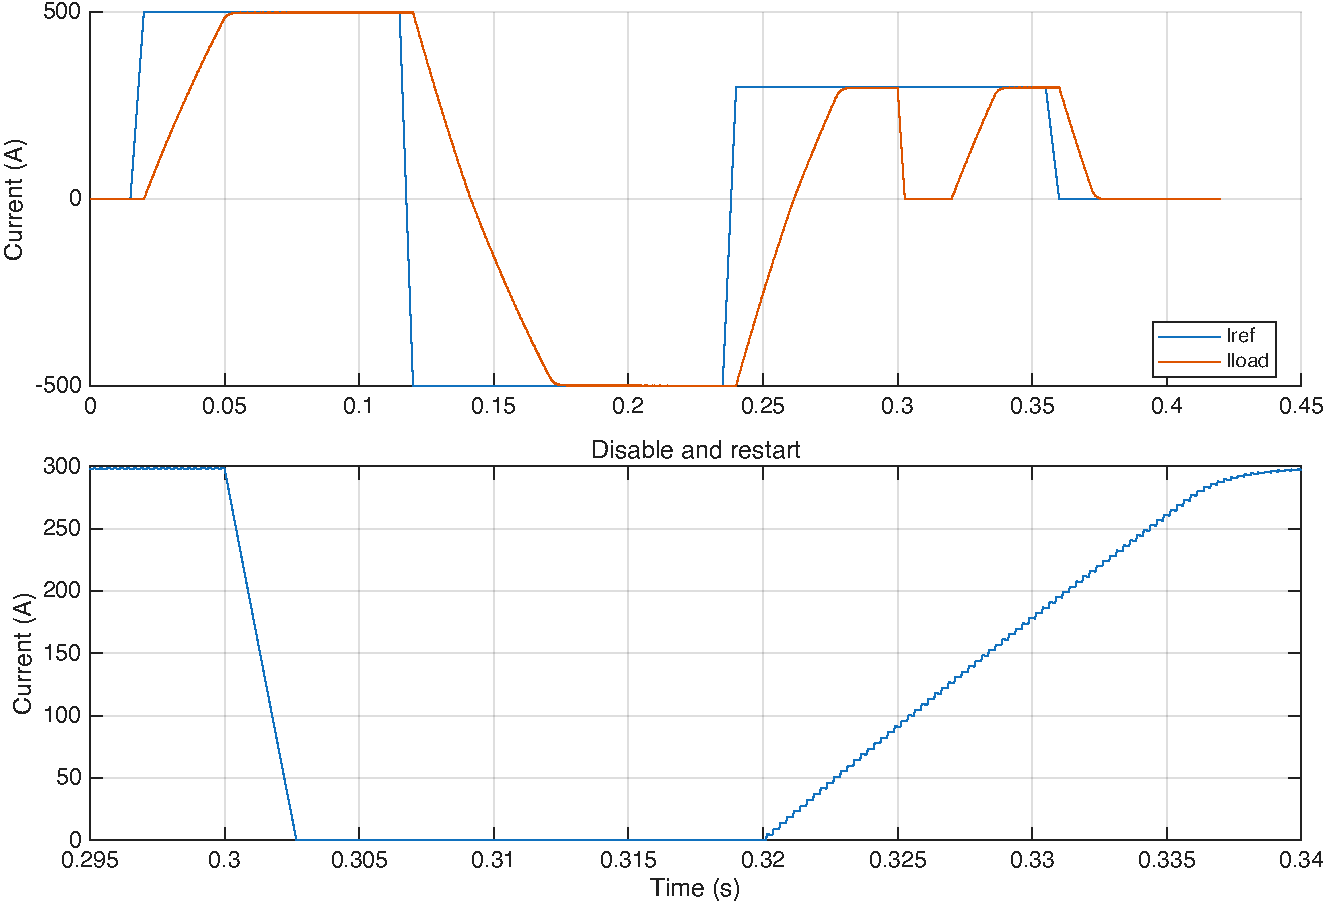
\includegraphics[width=0.68\linewidth]{native/verified_tracking_restart.pdf}
\caption{修正版模型的 MATLAB 原生波形：五段给定跟踪（上）与使能封锁、恢复过程（下）}
\label{fig:hb-tracking}
\end{figure}

\begin{dtable}{htbp}{五段工况的稳态跟踪结果}
\label{tab:hb-track}
\begin{tabularx}{\linewidth}{P{0.36\linewidth}RRRR}
\toprule
\headrow 工况 & $\overline{i\sub{ref}}$ / A & $\overline{i\sub{load}}$ / A & 误差 / A & 纹波 / A \\
\midrule
0~A（0--0.02~s） & 0.03 & 0.000 & 0.03 & 0.00 \\
$+500$~A（0.02--0.12~s） & 500.00 & 499.32 & 0.68 & 1.64 \\
$-500$~A（0.12--0.24~s） & $-499.99$ & $-498.74$ & 1.25 & 1.71 \\
$+300$~A（0.24--0.30~s） & 300.00 & 298.23 & 1.77 & 1.15 \\
$+300$~A（使能 $=0$，0.30--0.32~s） & 300.00 & 0.00 & --- & 0.00 \\
$+300$~A（复位后，0.32--0.36~s） & 300.00 & 298.64 & 1.36 & 1.03 \\
0~A（0.36--0.42~s） & 0.00 & 0.0003 & 0.0003 & 0.0003 \\
\bottomrule
\end{tabularx}
\end{dtable}

方向和幅值都正确，说明电流测量极性、环路符号和 $v\sub{AB}\propto m\sub{H}$ 三者一致。残差的量级也可以解释：死区每个周期造成约 17.6~V 的电压损失，由积分器补偿，而误差通道带有被控对象极点 $s=-R/L$（时间常数 100~ms），残差按 100~ms 衰减。$+500$~A 平台长 100~ms，残差降到 0.68~A；$+300$~A 平台只有 60~ms，结束时还有 1.77~A 且仍在下降。阶跃响应没有超调，$+500$~A 段峰值为 500.12~A，抗饱和起到了作用。

\section{两条独立关系的校核}

把 1~$\mu$s 波形按 500~$\mu$s 分成 840 个窗口，每个窗口对 $v\sub{AB}$、$m\sub{H}$ 和电流取平均。

第一条是调制律。稳态窗口里 $\langle v\sub{AB}\rangle-U\sub{dc}\langle m\sub{H}\rangle$ 的幅值中位数为 18.40~V（正电流段中位数 $-20.0$~V，负电流段 $+18.5$~V），而死区损失为
\begin{equation}
\Delta v=\pm U\sub{dc}\frac{2t_d}{T_s}=\pm2200\times\frac{2\times2\ \mu\mathrm{s}}{500\ \mu\mathrm{s}}=\pm17.60\ \mathrm{V}.
\label{eq:dtvolt}
\end{equation}
偏差符号由电流方向决定，幅值与式~\eqref{eq:dtvolt} 相符（图~\ref{fig:hb-dtvolt}）。按 17.60~V 补偿后残差均方根 7.98~V、最大 14.53~V，不超过 $U\sub{dc}$ 的 0.66\%，其余部分来自器件压降、$m\sub{H}$ 的 50~$\mu$s 离散化和窗口边界效应。

\begin{figure}[htbp]
\centering
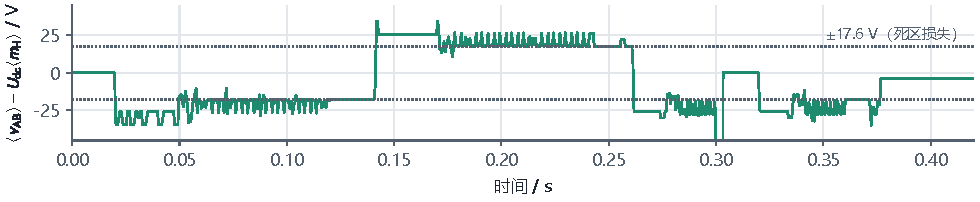
\includegraphics[width=\linewidth]{hb_deadtime_voltage}
\caption{开关周期平均的 $\langle v\sub{AB}\rangle-U\sub{dc}\langle m\sub{H}\rangle$ 在死区损失 $\pm17.6$~V 附近呈台阶状，符号随电流方向改变}
\label{fig:hb-dtvolt}
\end{figure}

第二条是负载回路方程式~\eqref{eq:rl}。对周期平均值做数值微分后，稳态窗口残差的中位数为 0.00~V、均方根为 2.85~V；全部 840 个窗口的最大残差 565~V 出现在阶跃瞬间，属于用窗口平均近似微分的离散化误差。

使能封锁段需要单独解释（图~\ref{fig:hb-tracking} 下）。使能置零后四路门极全为 0，积分状态清零；同臂两管都关断后，感性电流经反并联二极管回馈直流侧，$v\sub{AB}$ 被钳到 $-2204$~V（$-U\sub{dc}$ 减两个二极管压降），电流按 $(-2204-Ri)/L\approx-115$~kA/s 下降，约 2.7~ms 降到零，远快于 $RL$ 无源放电的 100~ms 时间常数。这一段把“控制器复位”和“主电路断开”区分开来：若把封锁理解成断开，就无法解释实测的衰减速度。0.32~s 使能恢复后，电流在 40~ms 内重新跟到 298.64~A。
